\subsection{}

Data can be collected through the real world or simulations. 
One type of data is called an index set of data or index number.
\begin{example}
    Consumer Price Index (CPI) is an index number that measures the average price of a basket of goods and services purchased by households.
\end{example}
An index number is trying to present a cost relative to a reference period for every hundred dollars. They can be used to measure inflation.
\begin{figure}[h!]
    \centering
    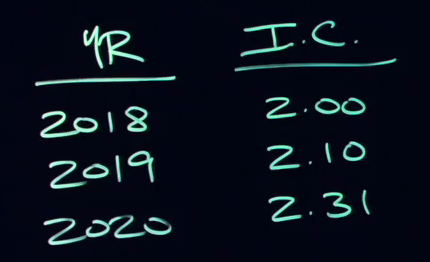
\includegraphics{Chapter2/IceCapCosts.png}
    \caption{Ice Cap Costs Over Three Years}
\end{figure}
\newpage
With an index, we need to select a \emph{base year}.
The base year influences the index number.

Let us assume 2018 is the base year.
\begin{figure}[h!]
    \centering
    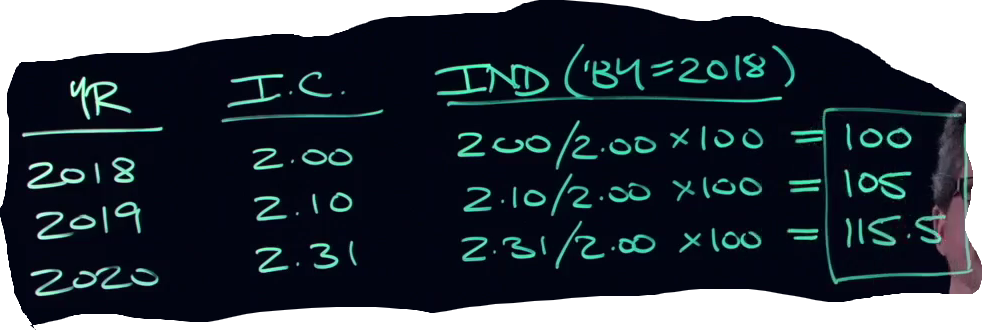
\includegraphics{Chapter2/IceCapIndex.png}
    \caption{Index of Ice Cap Costs Over Three Years, with 2018 as the base year}
\end{figure}
\begin{equation}
    \text{Index} = \frac{\text{Cost in Year X}}{\text{Cost in Base Year}} \times 100
\end{equation}
Composite index is an index made up of multiple items.

Data type sets commonly come in two forms:
\begin{itemize}
    \item \begin{definition}
        \emph{Time series data}, looking at particular data over a period of time.
    \end{definition}
    \item \begin{definition}
        \emph{Cross-sectional data}, looking at a snapshot of data at a particular point in time.
    \end{definition}
\end{itemize}